\documentclass[11pt]{article}
\usepackage[a4paper,margin=2.5cm]{geometry}
\usepackage[T1]{fontenc}
\usepackage[utf8]{inputenc}
\usepackage{amsmath,amssymb}
\usepackage{booktabs,array}
\usepackage{graphicx}
\usepackage{xcolor}
\usepackage[numbers,sort&compress]{natbib}
\usepackage[colorlinks=true,linkcolor=blue!50!black,citecolor=blue!50!black,urlcolor=blue!50!black]{hyperref}
\graphicspath{{../../examples/}}

\newcommand{\qgZ}{qg_Z}
\newcommand{\qgX}{qg_X}
\newcommand{\qgY}{qg_Y}

\title{Storing energy and sharing entanglement, read in qg:\\
a charging rule for qubit batteries and a slot rule for Bell-pair distillation}
\author{Vicente Humberto Monteverde\\
\small Universidad del Museo Social Argentino (UMSA), Argentina\\
\small ORCID 0000-0001-8884-4811}
\date{\small Draft of 27 September 2026}

\begin{document}
\maketitle

\begin{abstract}
Qubit batteries and Bell pairs stored in network memories both age under the same two
processes, relaxation (T1) and dephasing (T2). Both are also judged by a few expectation values:
the polar bias $\qgZ=\langle\sigma_z\rangle$ and its companions $\qgX,\qgY$~\cite{monteverde2026qang}
for a battery, and three correlations $c_x,c_y,c_z$ with two local polar biases for a pair. We
write both problems in these measured quantities and ask what practical rules follow. (i) For a
qubit battery the ergotropy is $W=(\omega/2)(r-\qgZ)$, with $r$ the Bloch length. A battery used
before the time $t_c$ should be charged fully; after it, it should be tilted, to about $0.6\pi$ at
$t=T_1$. The crossover solves $x^{2T_1/T_2-1}=2(2x-1)$ with $x=e^{-t_c/T_1}$. Coherence buys storage
time only when $T_2$ is comparable to $T_1$. Certifying the stored work from shots is expensive: the
plug-in estimate reports work in a passive state in every run, and a safe bound with 1000 shots per
axis certifies 40\% of it. A Dicke register stores charge that no single qubit can release, and the
register-mean $\qgZ$ cannot see this, while the sum of local ergotropies can. (ii) For a Bell pair,
each Pauli noise leaves one correlation at its ideal value, and only memory T1 moves the local polar
biases, which gives a T1 witness on a shared pair. The textbook DEJMPS order can lower the
fidelity (0.820 to 0.705 under Y-flip noise); putting the smallest error estimated from 200 shots per
setting in the combined slot reaches the best output. For BBM92 with stored pairs, the latest usable
storage time has a closed form in the aged correlations, and one distillation round roughly doubles
it. All results are simulations, reproduced by scripts and pinned by regression tests.
\end{abstract}

\section{Two problems, one description}

A qubit battery with Hamiltonian $H=\omega|1\rangle\langle1|$ and a Bell pair waiting in two
memories age under the same channels. Amplitude damping with $g=1-e^{-t/T_1}$ moves populations
towards $|0\rangle$, and dephasing shrinks coherences as $e^{-t/T_2}$. The questions differ: how much
work can still be extracted, and whether a pair is still good enough to distil or to use for a key.
In both cases the answer depends on a handful of expectation values, and those are the numbers an
experiment measures. This note collects what the qg description of these values gives in practice,
and states which parts are known.

\section{Qubit batteries}\label{sec:battery}

\paragraph{Ergotropy in qg.} A qubit with Bloch vector $(\qgX,\qgY,\qgZ)$ of length $r$ stores
energy $\omega(1-\qgZ)/2$. Its ergotropy~\cite{allahverdyan2004}, the work a unitary can extract, is
\begin{equation}\label{eq:ergo}
W=\frac{\omega}{2}\,(r-\qgZ)=W_{\rm inc}+W_{\rm coh},\qquad
W_{\rm inc}=\omega\max(0,-\qgZ),\quad W_{\rm coh}=\frac{\omega}{2}\,(r-|\qgZ|).
\end{equation}
It agrees with the general eigenvalue formula to $3\times10^{-16}$ on 200 random states, and the
storage curves below agree with an integrated Lindblad equation.

\paragraph{Storage and the charging rule.} A battery charged at polar angle $\theta$ ages as
$\qgZ(t)=1-(1-\cos\theta)e^{-t/T_1}$ and $r_\perp(t)=\sin\theta\,e^{-t/T_2}$.
Table~\ref{tab:battery} gives the best angle and the ergotropy for three strategies. Full charging
($\theta=\pi$) is best if the battery will be used before a crossover time $t_c$. After $t_c$ a tilted
battery stores more, because the inverted one stops storing anything at $t=T_1\ln2$, while the
coherent part decays with $T_2$. A small-tilt analysis gives
\begin{equation}\label{eq:tc}
x^{2T_1/T_2-1}=2(2x-1),\qquad x=e^{-t_c/T_1},
\end{equation}
which matches the numerical optimum to $10^{-6}$ and tends to $T_1\ln2$ as $T_2$ shrinks.

\begin{table}[t]
\centering\small
\caption{Qubit battery storage. Best angle and ergotropy (best / fully inverted / equator), in units
of $\omega$.}
\label{tab:battery}
\begin{tabular}{lcccc}
\toprule
$T_2/T_1$ & $t_c$ & $t=0.5\,T_1$ & $t=T_1$ & $t=2\,T_1$\\
\midrule
2 & $0.288\,T_1=\ln(4/3)$ & $0.70\pi$: .297 / .213 / .240 & $0.58\pi$: .129 / 0 / .122 & .038 / 0 / .038\\
1 & $0.405\,T_1=\ln(3/2)$ & $0.78\pi$: .234 / .213 / .165 & $0.59\pi$: .054 / 0 / .050 & .005 / 0 / .005\\
0.5 & $0.618\,T_1$ & $\pi$: .213 / .213 / .073 & $0.60\pi$: .008 / 0 / .007 & $\approx0$\\
0.2 & $0.692\,T_1$ & $\pi$: .213 / .213 / .004 & $\approx0$ & $\approx0$\\
\bottomrule
\end{tabular}
\end{table}

The practical reading is short. Charge fully if the battery will be used before $t_c$; otherwise
tilt it, to about $0.6\pi$ at $t=T_1$. At $t=T_1$ the tilted battery stores $0.13\,\omega$ for
$T_2=2T_1$ and $0.05\,\omega$ for $T_2=T_1$, where the inverted one stores nothing. At $T_2=0.2\,T_1$
coherence buys nothing. Platforms without relevant T1 on the storage time scale, such as trapped-ion
qubits, should always charge fully.

\paragraph{Certifying the stored work.} Eq.~\eqref{eq:ergo} needs $r$, and $r$ comes from three
estimated components. Shot noise in each inflates $r$, so the plug-in estimate overestimates $W$ in
more than half of the runs and reports positive ergotropy for a passive state in every run. A
$3\sigma$ lower bound is never unsafe, but it is costly: with 1000 shots per axis it certifies
$0.086$ of $0.213\,\omega$, and nothing for a nearly discharged battery.

\paragraph{Locked charge in registers.} For $n=4$ qubits with two excitations and $T_2=T_1$, the Dicke
state $D(4,2)$ stores $2\omega$, all of it globally extractable, but each qubit alone is passive
($\qgZ=0$, no coherence). The sum of local ergotropies is 0 for the Dicke battery and $2\omega$ for a
product battery with the same energy. The register mean of $\qgZ$ is the same for both and cannot tell
them apart; the local sum can. The locked charge is also more fragile under local noise: $0.71$ vs
$1.05\,\omega$ at $0.3\,T_1$, and $0.05$ vs $0.41\,\omega$ at $0.7\,T_1$.

\begin{figure}[t]
\centering
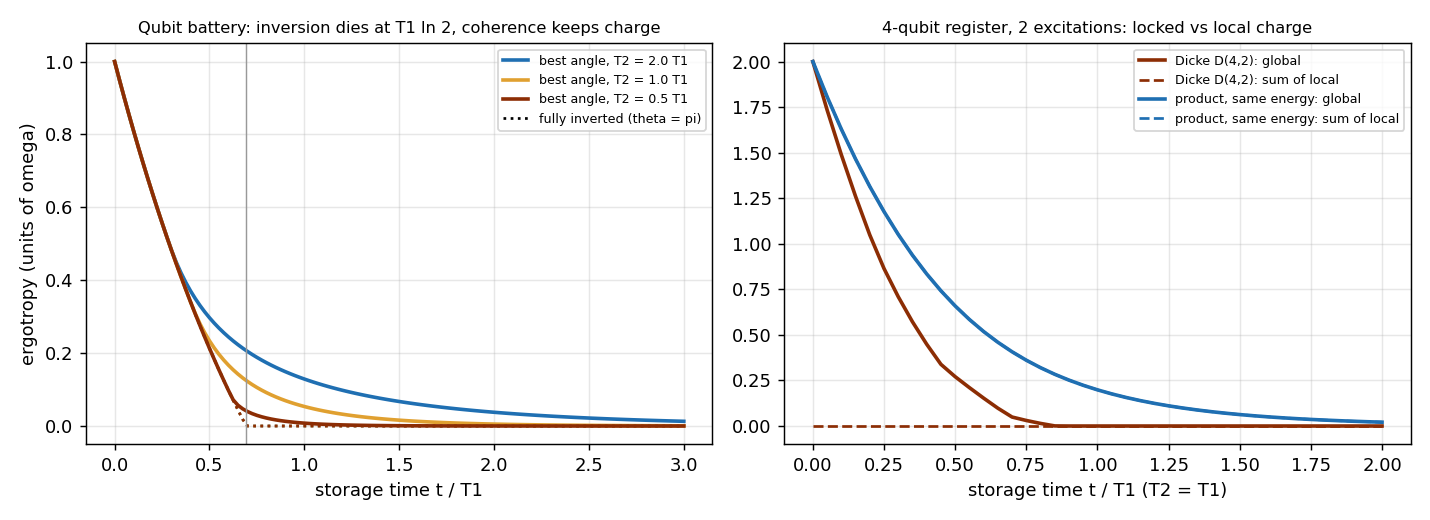
\includegraphics[width=\linewidth]{battery_ergotropy_qg.png}
\caption{Left: ergotropy at the best charging angle against storage time for three values of
$T_2/T_1$; the fully inverted battery is empty after $T_1\ln2$ (vertical line). Right: a 4-qubit
register with two excitations ($T_2=T_1$): global ergotropy and sum of local ergotropies for $D(4,2)$
and for a product battery with the same energy.}
\label{fig:battery}
\end{figure}

\section{Bell pairs in a network}\label{sec:bell}

\paragraph{Five numbers.} A pair meant to be $|\Phi^+\rangle$ is described by
$c_x=\langle XX\rangle$, $c_y=\langle YY\rangle$, $c_z=\langle ZZ\rangle$ and the local biases
$m_A=\langle Z_A\rangle$, $m_B=\langle Z_B\rangle$. Three measurement settings give all five. The
fidelity is exact for any state,
\begin{equation}\label{eq:fid}
F=\tfrac14\,(1+c_x-c_y+c_z),
\end{equation}
and the Bell-diagonal weights of the twirled pair,
$\Phi^-\!:(1-c_x+c_y+c_z)/4$, $\Psi^+\!:(1+c_x+c_y-c_z)/4$, $\Psi^-\!:(1-c_x-c_y-c_z)/4$, say which
error dominates: $\Phi^-$ is a phase flip, $\Psi^+$ a bit flip, $\Psi^-$ both.

\paragraph{Noise signatures.} Table~\ref{tab:sig} shows the five numbers for $p=0.1$ on each half.
Each Pauli noise keeps one correlation at its ideal value. Only amplitude damping, that is memory T1,
moves $m_A$ and $m_B$ away from zero. This is the T1 witness used for BB84 in the companion note on cryptography,
now on a shared pair, and it is read from the same $ZZ$ shots.

\begin{table}[t]
\centering\small
\caption{Noise signatures of a stored pair ($p=0.1$ on each half; amplitude damping $g=0.1$).}
\label{tab:sig}
\begin{tabular}{lcccccl}
\toprule
noise & $c_x$ & $c_y$ & $c_z$ & $m_A=m_B$ & $F$ & largest error\\
\midrule
dephasing & $+0.64$ & $-0.64$ & $\mathbf{+1.00}$ & 0 & 0.820 & $\Phi^-$\\
bit flip & $\mathbf{+1.00}$ & $-0.64$ & $+0.64$ & 0 & 0.820 & $\Psi^+$\\
Y flip & $+0.64$ & $\mathbf{-1.00}$ & $+0.64$ & 0 & 0.820 & $\Psi^-$\\
depolarizing & $+0.81$ & $-0.81$ & $+0.81$ & 0 & 0.858 & all equal\\
amplitude damping & $+0.90$ & $-0.90$ & $+0.82$ & $\mathbf{+0.10}$ & 0.905 & $\Psi^+$\\
\bottomrule
\end{tabular}
\end{table}

\paragraph{Which distillation.} The DEJMPS recurrence~\cite{deutsch1996} (a refinement of
Ref.~\cite{bennett1996}) combines the $\Phi^+$ weight $A$ with the error weight $B$ that sits in one
slot, $A'=(A^2+B^2)/N$, and local rotations choose which error goes there. Table~\ref{tab:dejmps}
compares the textbook slot ($\Psi^-$), the best slot, and a rule applied from data: put the smallest
error estimated from the three correlations, with 200 shots per setting, in slot $B$.

\begin{table}[t]
\centering\small
\caption{One DEJMPS round: output fidelity (success probability).}
\label{tab:dejmps}
\begin{tabular}{lcccc}
\toprule
input & $F_{\rm in}$ & textbook slot & best slot & qg rule, 200 shots/setting\\
\midrule
dephasing 0.1 & 0.820 & 0.954 (0.705) & 0.954 (0.705) & 0.954 (right slot 100\%)\\
bit flip 0.1 & 0.820 & 0.954 (0.705) & 0.954 (0.705) & 0.954 (100\%)\\
Y flip 0.1 & 0.820 & \textbf{0.705} (1.000) & 0.954 (0.705) & 0.954 (100\%)\\
depolarizing 0.1 & 0.858 & 0.891 (0.828) & 0.891 (0.828) & 0.891 (100\%)\\
amplitude damping 0.2 & 0.820 & 0.828 (0.820) & 0.920 (0.731) & 0.915 (94\%)\\
\bottomrule
\end{tabular}
\end{table}

The fixed order fails when the dominant error sits in the slot combined with $\Phi^+$. For Y-flip
noise one round lowers the fidelity, from 0.820 to 0.705, and for amplitude damping it gains almost
nothing (0.828 against a possible 0.920). The data-driven rule reaches the best output in every case,
94\% of the time for amplitude damping, where two error weights are close.

\paragraph{Memory cutoff for BBM92.} For entanglement-based key distribution~\cite{bbm92} with
QBER$_Z=(1-c_z)/2$, QBER$_X=(1-c_x)/2$ and secret fraction $1-h(\mathrm{QBER}_X)-h(\mathrm{QBER}_Z)$,
the aged correlations have closed forms,
\begin{equation}\label{eq:aged}
c_x=-c_y=e^{-2t/T_2},\qquad c_z=1-2g+2g^2,\qquad m=g,\qquad g=1-e^{-t/T_1},
\end{equation}
so the latest usable storage time follows directly (Table~\ref{tab:cutoff}). One distillation
round with the best slot roughly doubles it when T1 limits storage. It costs half the pairs, so per
raw pair it pays only after the crossover time in the last row.

\begin{table}[t]
\centering\small
\caption{Latest storage time with a positive BBM92 secret fraction, in units of $T_1$.}
\label{tab:cutoff}
\begin{tabular}{lcccc}
\toprule
$T_2/T_1$ & 2 & 1 & 0.5 & 0.2\\
\midrule
no distillation & 0.184 & 0.129 & 0.088 & 0.051\\
one DEJMPS round & 0.395 & 0.232 & 0.144 & 0.076\\
distilling pays per raw pair after & 0.085 & 0.083 & 0.056 & 0.032\\
\bottomrule
\end{tabular}
\end{table}

\begin{figure}[t]
\centering
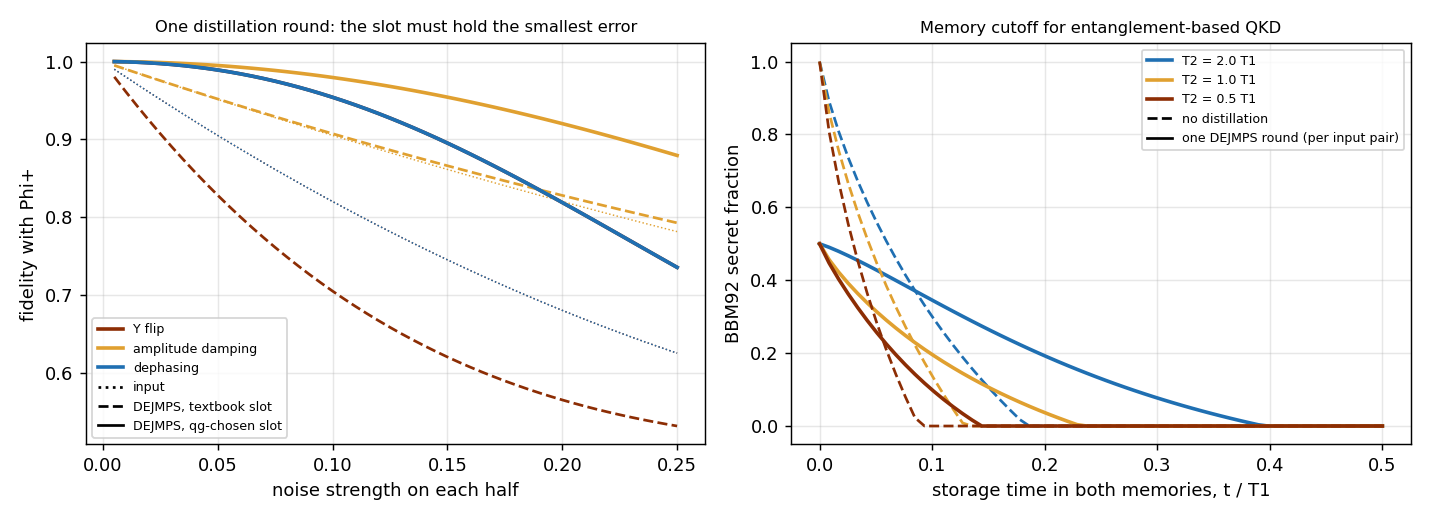
\includegraphics[width=\linewidth]{bell_pairs_network_qg.png}
\caption{Left: fidelity after one DEJMPS round against noise strength, with the textbook slot
(dashed) and the slot chosen from qg data (solid); dotted lines are the input. Right: BBM92 secret
fraction against storage time, without distillation (dashed) and after one round, per input pair
(solid).}
\label{fig:bell}
\end{figure}

\section{What is common}

Three points hold in both settings. First, T1 and T2 play different roles, and the ratio $T_2/T_1$
decides the rule: how far to tilt a battery, and how much a distillation round extends a pair's life.
Second, a local polar bias is a free T1 witness: $\qgZ$ of a stored battery and $m_A,m_B$ of a stored
pair come from shots already taken. Third, single-qubit or register-mean quantities miss what is
shared: the register mean of $\qgZ$ cannot see locked charge, and local biases cannot see which Bell
error dominates. The useful description keeps the local numbers and the few correlations that
matter.

\section{Limitations}

(i) Everything is simulation with independent Markovian T1 and T2 channels and perfect local gates; no
hardware data. (ii) Eq.~\eqref{eq:ergo}, coherence-assisted storage, locally passive but globally
charged batteries~\cite{alicki2013}, Eq.~\eqref{eq:fid}, the Bell-diagonal reading, DEJMPS with local
rotations and memory cutoffs are known. The contributions are the charging rule with its closed-form
crossover Eq.~\eqref{eq:tc}, the certification cost, the qg reading of which charge is locally
extractable, the noise signatures with the T1 witness on a pair, the slot rule applied from
finite-shot data, and the closed-form cutoff. (iii) Distillation uses the twirled state. (iv) The
BBM92 secret fraction is asymptotic; finite-key effects would shorten every cutoff in
Table~\ref{tab:cutoff}. (v) Charging and extraction are ideal unitaries; their cost and duration are
not modelled.

\section{Code availability}
\sloppy
\texttt{examples/battery\_ergotropy\_qg.py} and \texttt{examples/bell\_pairs\_network\_qg.py} in
\url{https://github.com/Viny2030/qang} (MIT license), with regression tests. Sections 56 and 57 of
\texttt{RESEARCH\_NOTES.md} give more detail.

\section*{Acknowledgments and use of AI tools}
Generative AI tools (Anthropic Claude Opus 5.5) assisted with code, numerical experiments, tests and
drafting. The author framed the questions, made the design decisions, and reviewed and validated all
AI-assisted output, including every number reported here.

\bibliographystyle{unsrtnat}
\bibliography{../refs}
\end{document}
